\documentclass[11pt,a4paper]{article}
%%%%%%%%%%%%%%%%%%%%%%%%% Credit %%%%%%%%%%%%%%%%%%%%%%%%

% template ini dibuat oleh martin.manullang@if.itera.ac.id untuk dipergunakan oleh seluruh sivitas akademik itera.

%%%%%%%%%%%%%%%%%%%%%%%%% PACKAGE starts HERE %%%%%%%%%%%%%%%%%%%%%%%%
\usepackage{graphicx}
\usepackage{caption}
\usepackage[protrusion=true, expansion=false]{microtype}
\usepackage{tabulary}
\usepackage{minted}
% \usepackage{amsmath}
\usepackage{fancyhdr}
% \usepackage{amssymb}
% \usepackage{amsthm}
\usepackage{placeins}
% \usepackage{amsfonts}
\usepackage{graphicx}
\usepackage[all]{xy}
\usepackage{tikz}
\usepackage{verbatim}
\usepackage[left=2cm,right=2cm,top=3cm,bottom=2.5cm]{geometry}
\usepackage{hyperref}
\usepackage{amsmath}
\hypersetup{
    colorlinks,
    linkcolor={red!50!black},
    citecolor={blue!50!black},
    urlcolor={blue!80!black}
}
\usepackage{caption}
\usepackage{subcaption}
\usepackage{multirow}
\usepackage{psfrag}
\usepackage[T1]{fontenc}
\usepackage[scaled]{beramono}
% Enable inserting code into the document
\usepackage{listings}
\usepackage{xcolor} 
% custom color & style for listing
\definecolor{codegreen}{rgb}{0,0.3,0}
\definecolor{codegray}{rgb}{0.5,0.5,0.5}
\definecolor{codepurple}{rgb}{0.7,0,0.7}
\definecolor{backcolour}{rgb}{0.9,0.9,0.9}
\definecolor{LightGray}{gray}{0.9}
\lstdefinestyle{mystyle}{
	backgroundcolor=\color{backcolour},   
	commentstyle=\color{green},
	keywordstyle=\color{codegreen},
	numberstyle=\tiny\color{codegray},
	stringstyle=\color{codepurple},
	basicstyle=\ttfamily\footnotesize,
	breakatwhitespace=false,         
	breaklines=true,                 
	captionpos=b,                    
	keepspaces=true,                 
	numbers=left,                    
	numbersep=5pt,                  
	showspaces=false,                
	showstringspaces=false,
	showtabs=false,                  
	tabsize=2
}
\lstset{style=mystyle}
\renewcommand{\lstlistingname}{code}
%%%%%%%%%%%%%%%%%%%%%%%%% PACKAGE ends HERE %%%%%%%%%%%%%%%%%%%%%%%%


%%%%%%%%%%%%%%%%%%%%%%%%% Data Diri %%%%%%%%%%%%%%%%%%%%%%%%
\newcommand{\student}{\textbf{Joshua Palti Sinaga (122140141)}}
\newcommand{\course}{\textbf{Teknologi Multimedia (IF4021)}}
\newcommand{\assignment}{\textbf{Tugas Besar}}

%%%%%%%%%%%%%%%%%%% using theorem style %%%%%%%%%%%%%%%%%%%%
\newtheorem{thm}{Theorem}
\newtheorem{lem}[thm]{Lemma}
\newtheorem{defn}[thm]{Definition}
\newtheorem{exa}[thm]{Example}
\newtheorem{rem}[thm]{Remark}
\newtheorem{coro}[thm]{Corollary}
\newtheorem{quest}{Question}[section]
%%%%%%%%%%%%%%%%%%%%%%%%%%%%%%%%%%%%%%%%
\usepackage{lipsum}%% a garbage package you don't need except to create examples.
\usepackage{fancyhdr}
\pagestyle{fancy}
\lhead{Joshua Palti Sinaga (122140141)}
\rhead{ \thepage}
\cfoot{\textbf{Paint LiveCam}}
\renewcommand{\headrulewidth}{0.4pt}
\renewcommand{\footrulewidth}{0.4pt}

%%%%%%%%%%%%%%  Shortcut for usual set of numbers  %%%%%%%%%%%

\newcommand{\N}{\mathbb{N}}
\newcommand{\Z}{\mathbb{Z}}
\newcommand{\Q}{\mathbb{Q}}
\newcommand{\R}{\mathbb{R}}
\newcommand{\C}{\mathbb{C}}
\setlength\headheight{14pt}

%%%%%%%%%%%%%%%%%%%%%%%%%%%%%%%%%%%%%%%%%%%%%%%%%%%%%%%555
\begin{document}
\thispagestyle{empty}
\begin{center}
	
\includegraphics[scale = 0.15]{Figure/ifitera-header.png}
	\vspace{0.1cm}
\end{center}
\noindent
\rule{17cm}{0.2cm}\\[0.3cm]
Nama: \student \hfill Tugas Ke: \assignment\\[0.1cm]
Mata Kuliah: \course \hfill Tanggal: 31 Mei 2025\\
\rule{17cm}{0.05cm}
\vspace{0.1cm}

%%%%%%%%%%%%%%%%%%%%%%%%%%%%%%%%%%%%%%%%%%%%% BODY DOCUMENT %%%%%%%%%%%%%%%%%%%%%%%%%%%%%%%%%%%%%%%%%%%%%
\begin{center}
    \section*{Paint LiveCam}
    \subsection*{Aplikasi Menggambar Interaktif dengan \textit{Computer Vision}}
\end{center}
\vspace{0.5cm}

\section{Deskripsi Proyek}

Paint LiveCam merupakan aplikasi menggambar interaktif yang memanfaatkan teknologi \textit{computer vision} untuk memberikan pengalaman menggambar yang unik. Berbeda dengan aplikasi drawing konvensional yang menggunakan mouse atau stylus, aplikasi Paint LiveCam memungkinkan pengguna untuk menggambar langsung menggunakan gerakan jari tangan mereka melalui kamera webcam secara real-time. Dengan mengintegrasikan teknologi \textit{hand tracking} dan \textit{face detection} dari MediaPipe, proyek ini bertujuan untuk untuk menciptakan pengalaman menggambar yang interaktif terhadap pergerakan pengguna.

Aplikasi ini dibaungn dengan memiliki fitur-fitur seperti menggambar dengan gesture jari telunjuk ketika posisi ujung jari berada di atas ruas jari, kontrol UI menggunakan jari tengah, dan yang paling unik adalah fitur dimana gambar yang dibuat di dekat area wajah akan mengikuti pergerakan kepala pengguna secara real-time. 

\section{Teknologi yang Digunakan}

Proyek Paint LiveCam dikembangkan menggunakan berbagai teknologi dan library modern untuk mendukung fungsionalitas computer vision dan interaksi real-time:

\begin{itemize}
    \item \textbf{Python}: Bahasa pemrograman utama untuk pengembangan aplikasi
    \item \textbf{OpenCV (cv2)}: Library untuk pemrosesan gambar, manipulasi video, rendering antarmuka visual, dan operasi computer vision
    \item \textbf{MediaPipe}: Framework Google AI untuk hand tracking (deteksi 21 landmark jari) dan face detection dengan akurasi tinggi
    \item \textbf{NumPy}: Library untuk operasi array matematika dan manipulasi data gambar secara efisien
    \item \textbf{pygame}: Framework untuk manajemen audio dan efek suara
\end{itemize}

\section{Penjelasan Program}
\subsection{Arsitektur Umum dan Struktur File}
Aplikasi Paint LiveCam dibangun secara modular dengan cara membuat file terpisah untuk masing-masing fungsi program:

\begin{itemize}
\item \texttt{main.py}: File utama yang mengatur alur utama aplikasi dan menyelaraskan interaksi antar modul
\item \texttt{hand\_tracker.py}: Modul untuk deteksi dan tracking gerakan tangan
\item \texttt{face\_tracker.py}: Modul untuk deteksi dan tracking wajah
\item \texttt{drawing\_canvas.py}: Modul untuk manajemen canvas dan UI controls
\item \texttt{sound\_manager.py}: Modul untuk manajemen audio dan efek suara
\item \texttt{configurations.py}: File konfigurasi untuk seluruh pengaturan aplikasi
\end{itemize}

\subsection{Alur Kerja Utama Aplikasi}
\begin{enumerate}
\item Inisialisasi kamera dan komponen tracking
\item Capture frame dari webcam secara real-time
\item Deteksi tangan dan ekstraksi landmark jari
\item Deteksi wajah dan posisi center wajah
\item Proses posisi dan kondisi tangan untuk melakukan aksi
\item Update canvas dengan stroke baru atau pergerakan wajah
\item Render hasil akhir dengan overlay UI
\item Simpan atau reset canvas berdasarkan input pengguna
\end{enumerate}

\subsection{Modul Inti}
\subsubsection{Konfigurasi Global (\texttt{configurations.py})}
Modul ini menyimpan semua pengaturan aplikasi yang dapat dimodifikasi:

\begin{lstlisting}[language=Python, caption=Konfigurasi utama aplikasi]
# Display configuration
WINDOW_NAME = "Paint LiveCam"
WINDOW_SIZE = (860, 640)

# Hand tracking configuration
MAX_HANDS = 1
HAND_DETECTION_CONFIDENCE = 0.5
HAND_TRACKING_CONFIDENCE = 0.5

# Face tracking configuration
FACE_DETECTION_CONFIDENCE = 0.5

# Drawing settings
DEFAULT_DRAWING_COLOR = (0, 255, 255)  # Yellow
DEFAULT_LINE_THICKNESS = 4
CANVAS_OPACITY = 1

# Available drawing colors
DRAWING_COLORS = {
    "Yellow": (0, 255, 255),
    "Blue": (255, 0, 0),
    "Green": (0, 255, 0),
    "Red": (0, 0, 255),
    "Purple": (255, 0, 255),
    "Orange": (0, 165, 255),
    "White": (255, 255, 255),
    "Black": (0, 0, 0),
}
\end{lstlisting}

\subsubsection{Hand Tracking (\texttt{hand\_tracker.py})}
Modul ini bertugas untuk mendeteksi dan melacak posisi tangan menggunakan library MediaPipe:

\begin{lstlisting}[language=Python, caption=Implementasi hand tracking]
class HandTracker:
    def __init__(self):
        self.mp_hands = mp.solutions.hands
        self.hands = self.mp_hands.Hands(
            static_image_mode=False,
            max_num_hands=config.MAX_HANDS,
            min_detection_confidence=config.HAND_DETECTION_CONFIDENCE,
            min_tracking_confidence=config.HAND_TRACKING_CONFIDENCE
        )
    
    def find_hands(self, img, draw=None):
        imgRGB = cv2.cvtColor(img, cv2.COLOR_BGR2RGB)
        self.results = self.hands.process(imgRGB)
        
        if self.results.multi_hand_landmarks:
            for hand_landmarks in self.results.multi_hand_landmarks:
                self.mp_drawing.draw_landmarks(img, hand_landmarks, 
                                             self.mp_hands.HAND_CONNECTIONS)
        return img
    
    def find_position(self, img):
        hand_landmarks = []
        if self.results.multi_hand_landmarks:
            my_hand = self.results.multi_hand_landmarks[0]
            h, w, _ = img.shape
            for id, lm in enumerate(my_hand.landmark):
                cx, cy = int(lm.x * w), int(lm.y * h)
                hand_landmarks.append([id, cx, cy])
        return hand_landmarks
\end{lstlisting}

\subsubsection{Face Tracking (\texttt{face\_tracker.py})}
Modul ini mendeteksi wajah dan memberikan informasi posisi untuk fitur gambar mengikuti wajah:

\begin{lstlisting}[language=Python, caption=Implementasi face tracking]
class FaceTracker:
    def __init__(self):
        self.mp_face_detection = mp.solutions.face_detection
        self.face_detection = self.mp_face_detection.FaceDetection(
            min_detection_confidence=config.FACE_DETECTION_CONFIDENCE
        )
    
    def find_faces(self, img, draw=None):
        imgRGB = cv2.cvtColor(img, cv2.COLOR_BGR2RGB)
        self.results = self.face_detection.process(imgRGB)
        
        faces = []
        if self.results.detections:
            h, w, c = img.shape
            for detection in self.results.detections:
                bbox = detection.location_data.relative_bounding_box
                x, y, width, height = int(bbox.xmin * w), int(bbox.ymin * h), \
                                    int(bbox.width * w), int(bbox.height * h)
                
                face = {
                    'bbox': (x, y, width, height),
                    'center': (x + width//2, y + height//2),
                    'size': (width, height)
                }
                faces.append(face)
                
                if draw:
                    cv2.rectangle(img, (x, y), (x + width, y + height), (0, 255, 0), 2)
        
        return img, faces
\end{lstlisting}

\subsubsection{Drawing Canvas (\texttt{drawing\_canvas.py})}
Modul ini mengelola canvas drawing, UI, dan logika fitur garis mengikuti wajah:

\begin{lstlisting}[language=Python, caption=Ekstraksi posisi jari dan gesture recognition]
    def _extract_finger_positions(self, landmarks):
    """Extract index tip, index base, and middle tip positions from hand landmarks."""
    positions = {'index_tip': None, 'middle_tip': None, 'middle_one': None}
    
    for landmark_id, x, y in landmarks:
        if landmark_id == 8:    # Index finger tip
            positions['index_tip'] = (x, y)
        elif landmark_id == 12:  # middle finger tip
            positions['middle_tip'] = (x, y)
        elif landmark_id == 11: # middle finger book
            positions['middle_one'] = (x, y)
    
    return positions

    def _process_hand_input(self, positions):
    """Process hand gestures for drawing and UI interaction."""
    # Handle middle finger UI interaction
    if positions['middle_tip']:
        self.canvas.process_finger_input(positions['middle_tip'], 20)
    
    # Handle index finger drawing (only when tip is above base)
    if positions['index_tip'] and positions['middle_tip'] and positions['middle_one']:
        # disable drawing when V gesture is detected
        if positions['middle_tip'][1] > positions['middle_one'][1]:
            self.canvas.process_finger_input(positions['index_tip'], 8)
        else:
            self.canvas.stop_drawing(positions['index_tip'])
\end{lstlisting}

\paragraph{Garis Mengikuti Wajah}
Implementasi fitur dimana gambar dapat mengikuti pergerakan wajah:

\begin{lstlisting}[language=Python, caption=Implementasi face-following drawings]
def update_with_face_movement(self, face_center):
    if not self.last_face_center or not face_center or not self.face_following_segments:
        self.last_face_center = face_center
        return
    
    # Calculate face movement offset
    dx = face_center[0] - self.last_face_center[0]
    dy = face_center[1] - self.last_face_center[1]
    
    # Move all face-following segments
    for segment_index in self.face_following_segments:
        if segment_index < len(self.drawing_segments):
            segment = self.drawing_segments[segment_index]
            segment['points'] = [(x + dx, y + dy) for x, y in segment['points']]
    
    self.last_face_center = face_center
    self.draw_on_canvas()

def stop_drawing(self, end_point=None):
    if not self.is_drawing or not self.drawing_segments:
        self.is_drawing = False
        return
    
    current_segment = self.drawing_segments[-1]
    last_point = end_point if end_point else current_segment['points'][-1]
    
    if last_point:
        # Check if line ended near any face to set future line mode
        face_detected = any(
            face['bbox'][0] <= last_point[0] <= face['bbox'][0] + face['bbox'][2] and
            face['bbox'][1] <= last_point[1] <= face['bbox'][1] + face['bbox'][3]
            for face in self._current_faces
        )
        
        # Update face mode for future lines
        new_mode = "following" if face_detected else "still"
        if new_mode != self.current_face_mode:
            self.current_face_mode = new_mode
            print(f"Face mode: {new_mode}")
\end{lstlisting}

\paragraph{Kontrol UI}
Tombol untuk beberapa aksi dengan ujung jari tengah:

\begin{lstlisting}[language=Python, caption=Implementasi UI button system]
class Button:
    def __init__(self, x, y, width, height, color, text, action):
        self.x, self.y, self.width, self.height = x, y, width, height
        self.color, self.text, self.action = color, text, action
        self.is_pressed = False
    
    def is_clicked(self, point):
        return (self.x <= point[0] <= self.x + self.width and 
                self.y <= point[1] <= self.y + self.height)
    
    def draw(self, img):
        # Button background (darker when pressed)
        btn_color = (self.color[0] - 40, self.color[1] - 40, self.color[2] - 40) \
                   if self.is_pressed else self.color
        cv2.rectangle(img, (self.x, self.y), 
                     (self.x + self.width, self.y + self.height), btn_color, cv2.FILLED)
        
        # Center text on button
        text_size = cv2.getTextSize(self.text, cv2.FONT_HERSHEY_SIMPLEX, 0.5, 2)[0]
        text_x = self.x + (self.width - text_size[0]) // 2
        text_y = self.y + (self.height + text_size[1]) // 2
        cv2.putText(img, self.text, (text_x, text_y), 
                   cv2.FONT_HERSHEY_SIMPLEX, 0.5, (255, 255, 255), 2)
        return img
\end{lstlisting}

\subsubsection{Sound Manager (\texttt{sound\_manager.py})}
Modul ini mengelola efek audio selama interaksi pengguna:

\begin{lstlisting}[language=Python, caption=Implementasi sound management]
import pygame
import os

pygame.mixer.init()

# Load sounds
sounds = {
    'click': pygame.mixer.Sound("sfx/click.mp3"),
    'writing': pygame.mixer.Sound("sfx/writing.mp3"),
}

def play_background():
    pygame.mixer.music.load("sfx/backsound.mp3")
    pygame.mixer.music.play(-1)
    pygame.mixer.music.set_volume(0.5)

def play_click():
    if 'click' in sounds:
        sounds['click'].set_volume(0.5)
        sounds['click'].play()

def play_writing():
    global writingChannel
    if not writingChannel or not writingChannel.get_busy():
        sounds['writing'].set_volume(0.5)
        writingChannel = sounds['writing'].play()
\end{lstlisting}

\section{Fitur Utama Aplikasi}
Aplikasi Paint LiveCam memiliki berbagai fitur interaktif yang menarik. Salah satu fitur utama adalah kemampuan menggambar menggunakan jari telunjuk, di mana sistem mendeteksi posisi ujung jari telunjuk di atas pangkal jari sebagai kondisi untuk memulai proses menggambar. Selain itu, terdapat fitur inovatif yang memungkinkan gambar yang dibuat di dekat wajah pengguna untuk mengikuti pergerakan wajah secara real-time, memberikan pengalaman menggambar yang unik dan dinamis.

Aplikasi ini juga mendukung berbagai pilihan warna dengan menyediakan delapan opsi warna yang dapat dipilih menggunakan ujung jari tengah. Pengguna dapat menyesuaikan ketebalan garis dengan memilih dari empat tingkat ketebalan, yaitu Thin, Medium, Thick, dan Very Thick, sesuai kebutuhan. Untuk menyimpan hasil karya, aplikasi menyediakan fitur penyimpanan yang memungkinkan pengguna menyimpan gambar dengan latar belakang kamera dalam format PNG yang dilengkapi dengan timestamp.

Selain fitur visual, aplikasi ini juga dilengkapi dengan feedback audio yang memberikan efek suara saat pengguna menggambar atau mengklik tombol UI, sehingga meningkatkan interaktivitas dan pengalaman pengguna secara keseluruhan.

\section{Kesimpulan}

\FloatBarrier
    \begin{figure}[h]
        \centering
        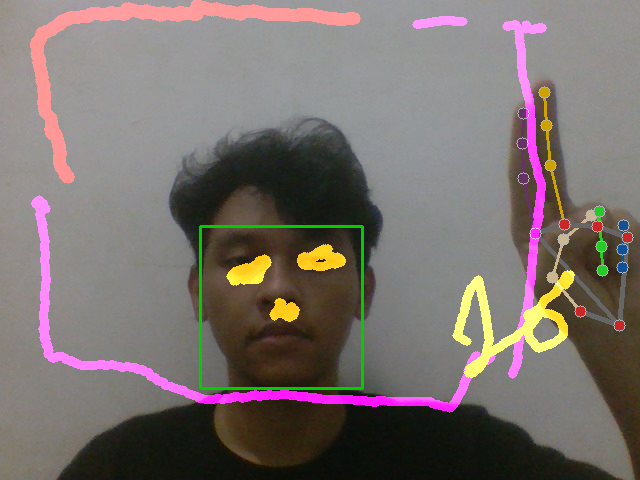
\includegraphics[width=0.8\textwidth]{Figure/demo.png}
        \caption{Tampilan Hasil save Gambar}
        \label{fig:demo_image}
    \end{figure}

    \begin{figure}[h]
        \centering
        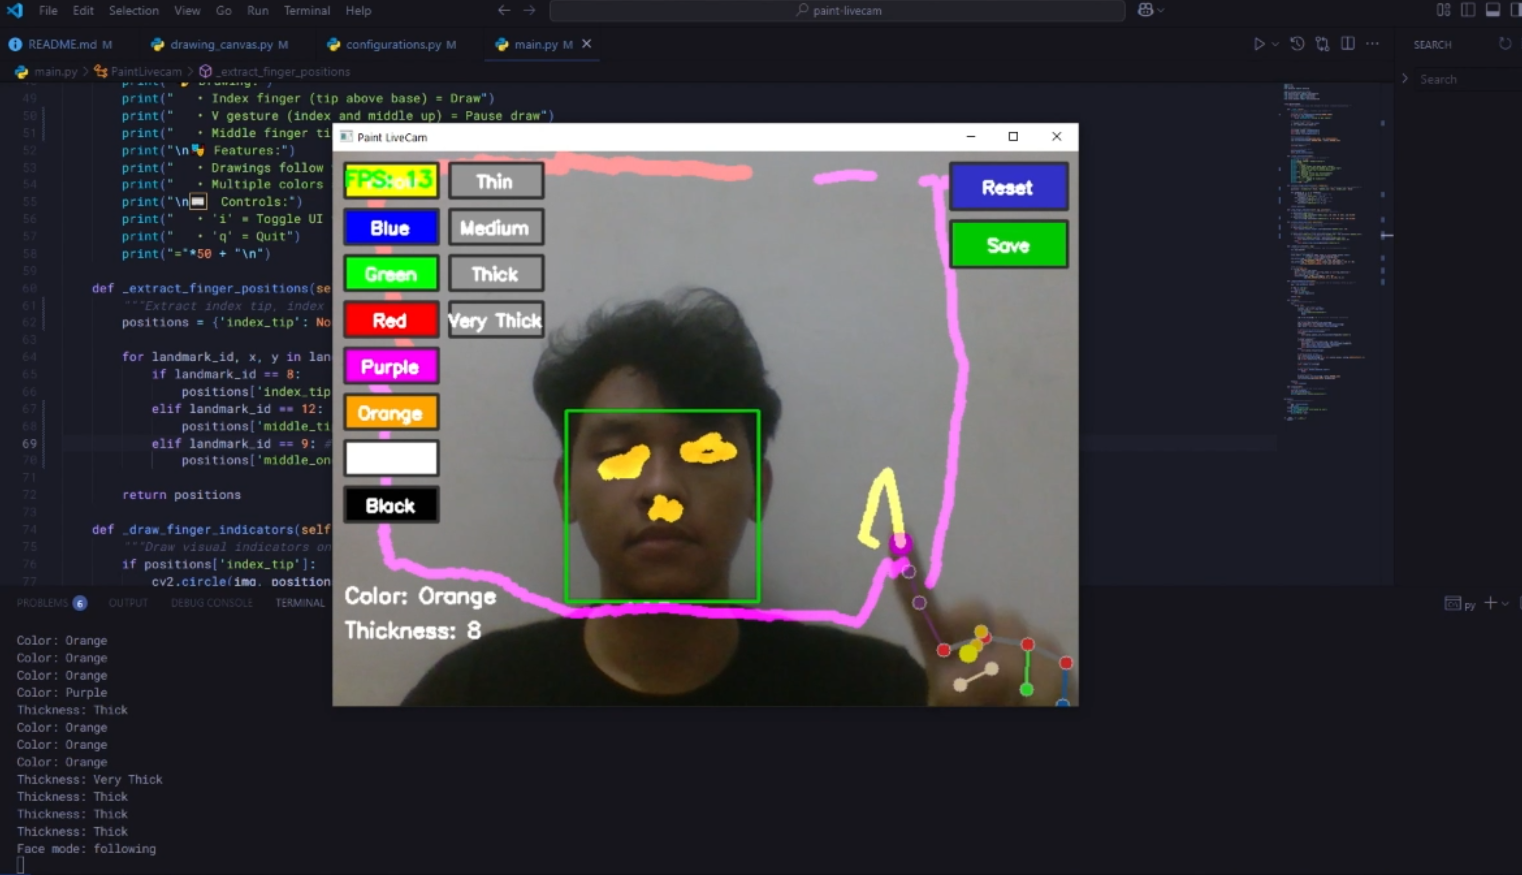
\includegraphics[width=0.8\textwidth]{Figure/ui.png}
        \caption{Tampilan Aplikasi Paint LiveCam}
        \label{fig:ui_image}
    \end{figure}
\end

Aplikasi Paint LiveCam berhasil mengimplementasikan sistem drawing interaktif menggunakan computer vision dengan fitur-fitur inovatif seperti face-following drawings. Aplikasi ini mendemonstrasikan integrasi sukses antara hand tracking, face detection, dan real-time image processing untuk menciptakan pengalaman pengguna yang intuitif dan menyenangkan. Fitur-fitur seperti gesture recognition, multi-color support, dan audio feedback menambah nilai interaktif dari aplikasi ini.

Proyek ini menunjukkan potensi besar penggunaan teknologi computer vision dalam aplikasi kreatif dan interaktif, serta memberikan fondasi yang solid untuk pengembangan lebih lanjut dalam bidang augmented reality dan human-computer interaction.

\section{Referensi}
\begin{enumerate}
\item MediaPipe Documentation. \textit{Hand Landmarks Detection}. Google AI. \url{https://google.github.io/mediapipe/solutions/hands.html}
\item MediaPipe Documentation. \textit{Face Detection}. Google AI. \url{https://google.github.io/mediapipe/solutions/face_detection.html}
\item OpenCV Documentation. \textit{OpenCV-Python Tutorials}. \url{https://docs.opencv.org/master/d6/d00/tutorial_py_root.html}
\item Zhang, F., et al. (2020). \textit{MediaPipe: A Framework for Building Perception Pipelines}. Google Research.
\end{enumerate}

\end{document}